Под информационной безопасностью объектов информатизации в общем случае понимается такое их состояние, при котором исключается нанесение неприемлемого ущерба субъектам информационных отношений при применении последними средств информатизации. Следовательно, для оценки информационной безопасности объектов информатизации важно оценить сначала степень информационной безопасности средств информатизации, применяемых на объектах информатизации, в том числе всех их компонентов.

Одной из важнейших составляющих любого объекта информатизации являются применяемые программные средства различного назначения, которые существенно влияют на информационную безопасность объекта информатизации в целом.

В настоящее время достаточно полно регламентирована законодательными актами и распорядительными документами организация работ по сертификации средств защиты информации. Разработаны и представлены в виде нормативных документов (Государственных стандартов и Руководящих документов Гостехкомиссии России) требования к защиты информации автоматизированных систем и их компонентов (вычислительных и программных средств). Отработаны методы их проверки и создано достаточно большое количество программных средств для проведения испытаний. Однако в основной их части требования касаются средств и методов защиты информации от несанкционированного доступа, а также проверок на отсутствие закладных деструктивных элементов в таких программных средствах.

В то же время информационная безопасность средств информатизации определяется не только их защищенностью от несанкционированного доступа. Одной из важнейших составляющих является выполнение средством информатизации заданных функций в различных условиях функционирования, в том числе при воздействии внешних деструктивных факторов.

Действительно, стержневой характеристикой качества любого средства информатизации является его функциональная пригодность. Ибо, если средство информатизации не решает в заданном объеме и с заданным качеством установленных для него задач, то нет смысла обеспечивать защиту от несанкционированного доступа и нецелесообразно его применять по назначению, так как только по этой причине результаты его использования могут привести к непредсказуемым последствиям и нанести пользователю неприемлемый ущерб.

В рамках Системы сертификации «Росинфосерт» разрабатывается подход к сертификации средств информатизации по требованиям информационной безопасности, сущность которого основана на действующей нормативно-методической базе Системы сертификации «Росинфосерт». Эта нормативно-методическая база дорабатывается с учетом требований Федерального закона «О техническом регулировании», в том числе в части вычислительных и программных средств, а также компьютерных систем в целом.

В ФЗ «О техническом регулировании» определены типы технических регламентов, в которых должны быть сформулированы требования по обеспечению биологической, механической, пожарной, промышленной, химической и др. видов безопасности применительно к продукции, работам и услугам. К сожалению, не попали в этот список требования по обеспечению информационной безопасности. Очевидно, Законодатель считает ее составной частью всех остальных видов безопасности.

Согласно закону, безопасность продукции определяется ее характеристиками, безопасность работ и предоставляемых услуг определяется применением безопасной продукции и безопасностью методов использования этой продукции при работах и предоставлении услуг. Фактически безопасность продукции является одной из составляющих ее качества.

Таким образом, информационная безопасность средств информатизации должна оцениваться в рамках общей оценки их качества, как один из показателей качества продукции.

При рассмотрении вопросов информационной безопасности исследуется и оценивается безопасность информационных ресурсов (данных, программ и их совокупности), которые, в свою очередь нельзя рассматривать в отрыве от вычислительных средств, на которых они размещены и реализованы. То есть предметом рассмотрения должны быть вычислительные средства с реализуемыми на них информационными ресурсами.

Таким образом, требования информационной безопасности следует применять к многоуровневому программно-вычислительному комплексу как единому целому (рисунок \ref{mnogour_pvk:pon1}):

\begin{figure}[h!]
\center{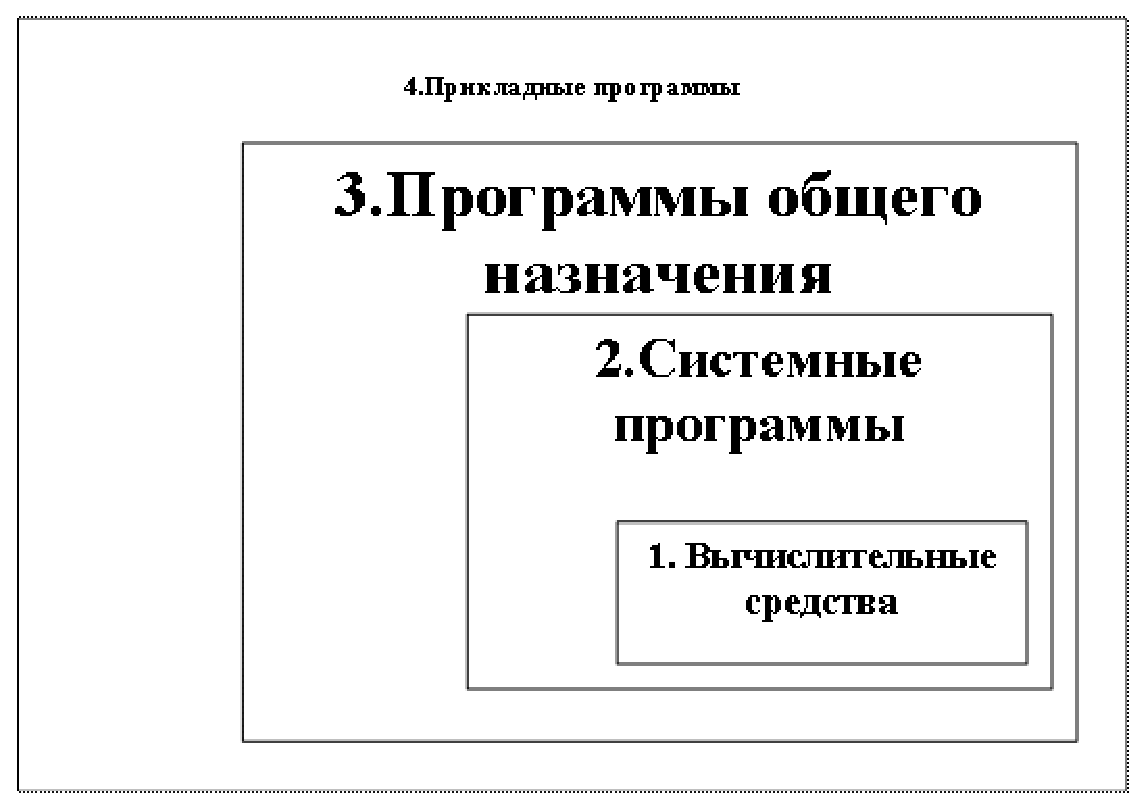
\includegraphics[width=0.6\linewidth]{pon1}}
\caption{Многоуровневый программно-вычислительный комплекс}
\label{mnogour_pvk:pon1}
\end{figure}

В характеристики качества (в том числе и в информационную безопасность) такого комплекса компоненты каждого уровня вносят свою составляющую. Например, недостаточная надежность технических компонентов вычислительных средств может компенсироваться программно-алгоритмическими решениями. В конечном счете, следует рассматривать в качестве основного показателя качества комплекса безопасность его функционирования.

Поскольку 100\% безопасности функционирования любого комплекса определенной структуры быть не может, то можно говорить о безопасности комплекса лишь в вероятностном смысле. Это в полной мере относится к компонентам любого уровня.

В общем случае для прикладных программных средств безопасное функционирование означает:

\begin{itemize}
\item полное и точное выполнение всех заданных функций;
\item обеспечение целостности и сохранности;
\item обеспечение защиты от неправильных действий пользователя, от некорректных входных данных, от случайных сбоев вычислительных средств;
\item простой и удобный интерфейс.
\end{itemize}

Эти составляющие обеспечивают как аппаратные средства, так и операционная среда, Однако, центральным моментом оценки качества прикладных программных средств должна являться оценка их собственных функциональных характеристик, но, прежде, чем провести оценку качества прикладных программных средств, следует убедиться в том, что характеристики остальных составляющих комплекса соответствуют предъявляемым к ним требованиям, в том числе требованиям информационной безопасности.

В свете всего сказанного предлагается следующая этапность оценки:

1-й этап – осуществляется оценка выполнения требований к качеству комплекса на первом уровне. Здесь исследуются и оцениваются характеристики преимущественно технических средств с использованием широкой номенклатуры специальных или специализированных тестов.

2-й этап – осуществляется оценка уже программно – аппаратного комплекса, включающего средства 1-го и 2-го уровней (технические средства и системные программные средства). При исследованиях и оценках используются имитаторы (в том числе программные) сигналов внешних устройств и функционирования программ общего назначения.

3-й этап – осуществляется оценка программно – аппаратного комплекса, включающего средства 1-го, 2-го и 3-го уровней (технические средства, системные программные средства и программные средства общего назначения). При оценках также используются независимые имитаторы сигналов внешних устройств, функционирования программ общего назначения и прикладных программ.

И, наконец, на 4-м этапе осуществляется оценка характеристик качества всего программно-вычислительного комплекса в целом. При этом используются результаты всех предыдущих этапов, что повышает достоверность и доверие к полученным оценкам.

Обязательные требования к продукции (работам и услугам) по действующему законодательству Российской Федерации устанавливаются Техническими регламентами, принимаемыми в качестве Федеральных законов. Сегодня необходимость технического регламента, устанавливающего обязательные требования по информационной безопасности к программно-вычислительным комплексам очевидна. При этом основным инструментом контроля соблюдения таких требований является сертификация (подтверждение соответствия). Место Системы сертификации в рамках проведения единой технической политики России в области решения задач информатизации поясняется рисунком \ref{sistsert:pon2}.

\begin{figure}[h!]
\center{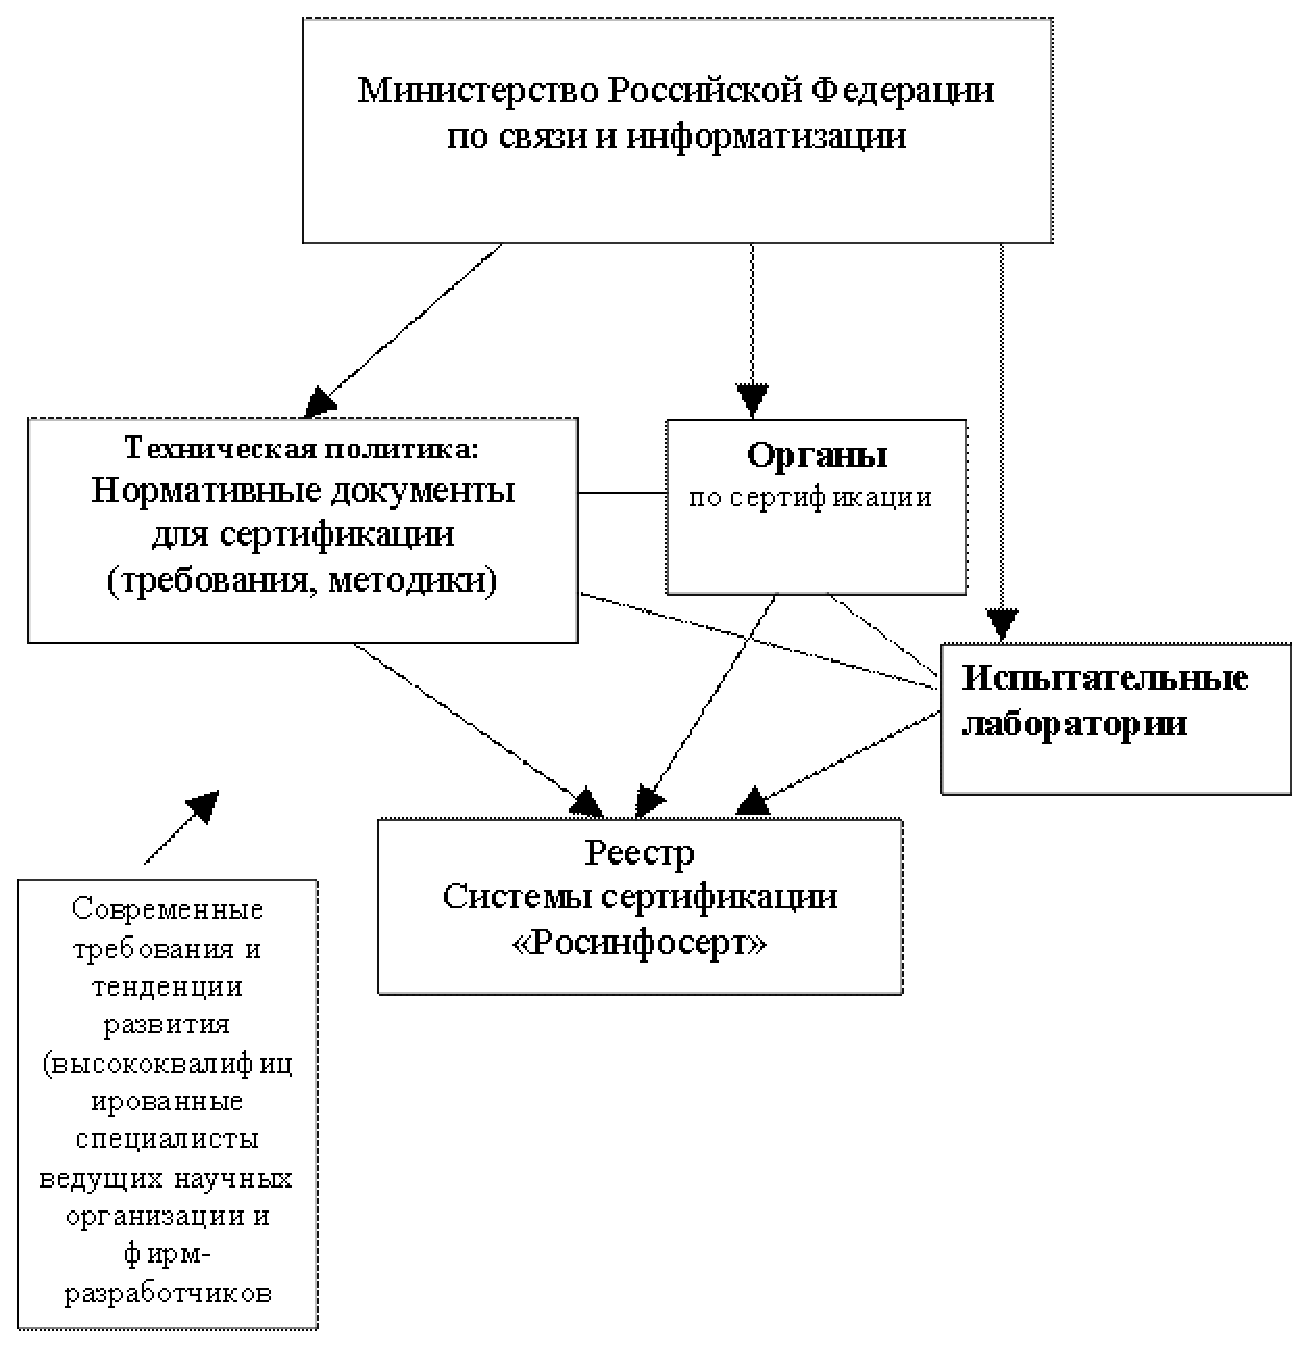
\includegraphics[width=0.8\linewidth]{pon2}}
\caption{Cистема сертификации при проведении единой технической политики}
\label{sistsert:pon2}
\end{figure}

Регистрация в реестре Системы сертифицированной продукции и выдача сертификата соответствия заявителю.
Применение результатов сертификации продукции можно проиллюстрировать примером проведения тендера на поставку средств информатизации для государственных нужд. Схема проведения такого тендера представлена на рисунке \ref{tender:pon3}.

\begin{figure}[h!]
\center{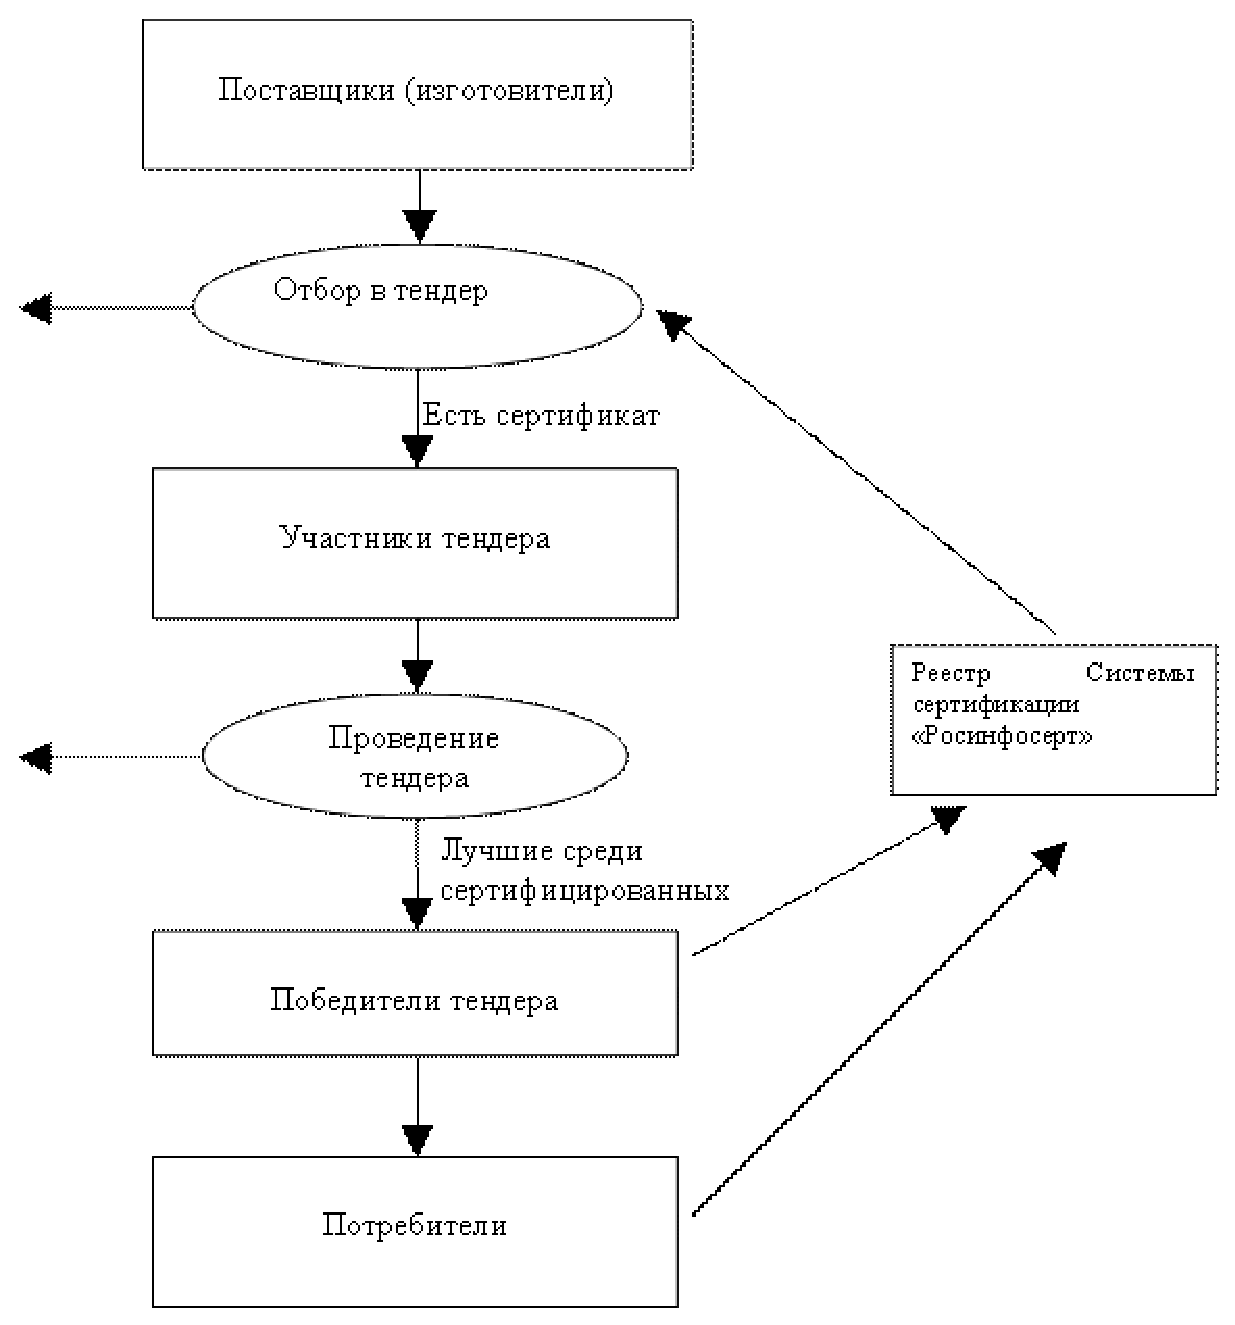
\includegraphics[width=0.8\linewidth]{pon3}}
\caption{Схема проведения тендера на поставку средств информатизации для государственных нужд}
\label{tender:pon3}
\end{figure}

Отбор участников тендера целесообразно проводить на основе анализа результатов их деятельности, одним из объективных показателей которой является сертификат соответствия системы менеджмента качества организации требованиям международных стандартов ИСО 9001 – 2001, а также наличие в номенклатуре выпускаемой продукции сертифицированных продуктов, характеристики которых представлены в Реестре Системы. Такой подход ставит барьер недобросовестным поставщикам и некачественной продукции на рынок средств информатизации России.

В этом случае нормативно-правовое обеспечение применения сертификации для реализации обязательных требований информационной безопасности составляют следующие документы:

\begin{enumerate}
\item Соглашение о взаимодействии в области сертификации средств информатизации между Минсвязи России и субъектом равного уровня. Такое соглашение является необязательным, но желательным документом, который регламентирует взаимоотношения руководства Системы сертификации, ее органов и испытательных лабораторий с потенциальными поставщиками и потребителями средств информатизации, впрямую не подчиняющимися Минсвязи России.
\item Распоряжение (постановление, приказ) субъекта об утверждении Положения о порядке использования средств информатизации для решения своих задач.
\item Положение о порядке использования субъектом средств информатизации, устанавливающее систему показателей и правил отбора и применения поставляемых для государственных нужд средств информатизации.
\item Нормативный документ для сертификации, содержащий состав характеристик средства информатизации, их допустимые значения и способы оценки. Этот документ носит статус стандарта организации, утверждается Минсвязи России по согласованию с субъектом.
\end{enumerate}
